\documentclass{article}

\usepackage{mathptmx}
%packages for language
\usepackage[czech]{babel}
\usepackage[utf8]{inputenc}
%packages for graphic
\usepackage{graphicx}
\usepackage{pgfplots}
\usepackage{pgfplotstable}
\usepackage{multirow}
\usepackage{tikz}
\usepackage{import}
\usepackage[a4paper, total={17cm,25.7cm}, top=2cm, left=2cm, includefoot]{geometry}
\usepackage{todonotes}
\usepackage{standalone}
\usepackage{colortbl}%pro barevne zmeny v tabulce
\usepackage{float}
\usepackage{csvsimple} %pro import a práci s csv soubory
\usepackage{indentfirst}  % odsazení prvního řádku v odstavci
\usepackage{hyperref} %dela odkazy na mista v dokumentu atd
\usepackage{amsmath}%psani matic
\usepackage{mathrsfs}%psani kroucenym matematickym pismem
\usepackage{pdfpages}%vkladani celych pdf dokumentu
\usepackage{caption}
\usepackage{subcaption}
%cesta k obrazkum: ./Graphics/....

\begin{document}
	\begin{titlepage}
    \begin{center}
        \LARGE
        Západočeská Univerzita v Plzni\\
        Fakulta Aplikovaných Věd\\
        
        \vspace{1cm}
        
        \includegraphics[width=0.5\textwidth]{./Graphics/FAV_logo.pdf}
        
        \vspace{4cm}
        
        \textbf{Markovské řetězce}
        
        \vspace{0.5cm}
        Semestrální práce č. 1
        
        \vspace{0.5cm}
        Filip Jašek
        
    \end{center} 
    \vfill
        \noindent
        \large
        Předmět: KKY/STP (Stochastické Systémy a Procesy)\\
        Přednášející: Doc. Ing. Straka Ondřej, Ph.D.\\
        Cvičící: Ing. Kost Oliver\hfill Datum: \today
\end{titlepage}
	
	\includepdf[scale=0.85,pages=1, pagecommand=\section{Zadání}\centering]{./Graphics/STP_semestralka02_zadani.pdf}
	
	\section{Příklad č. 1}
		\subsection{Teoretický výpočet kovarianční funkce}
			Pro zjištění obecné kovarianční funkce je potřeba určit několik prvních kovariancí. Pro následující výpočty bude užitečný vztah \[VAR[X_{k}]=E[X_{k}^{2}]+E[X_{k}]^{2},\] přičemž známe ze zadání hodnotu \(E[X_{k}]^{2}=0\), pak tedy známe \[E[X_{k}^{2}]=VAR[X_{k}]=Q.\]\\
			První kovariance:
			\begin{align}
				COV[X_{k+1},X_{k+1}] =& VAR[X_{k+1}]=VAR[e^{-bT}\cdot X_{k}+W_{k}] \\
 				COV[X_{k+1},X_{k+1}] =& e^{-2bT}VAR[X_{k}] + VAR[W_{k}]\\
 				COV[X_{k+1},X_{k+1}] =& Q\cdot e^{-2bT} + Q\cdot (1-e^{-2bT})\\
 				COV[X_{k+1},X_{k+1}] =& Q\cdot (e^{-2bT} + 1 - e^{-2bT})\\
 				COV[X_{k+1},X_{k+1}] =& Q = 3
			\end{align}
			Druhá kovariance:
			\begin{align}
				COV[X_{k},X_{k+1}] =& E[X_{k}\cdot X_{k+1}]+E[X_{k}]\cdot E[X_{k+1}]=E[e^{-bT}\cdot X_{k}^{2}+X_{k}\cdot W_{k}] \\
				COV[X_{k},X_{k+1}] =& e^{-bT}E[X_{k}^{2}] + E[X_{k}\cdot W_{k}]\\
				COV[X_{k},X_{k+1}] =& Q\cdot e^{-bT}
			\end{align}
			A analogicky další:
			\begin{align}
				COV[X_{k},X_{k+2}] =& Q\cdot e^{-2bT}\\
				COV[X_{k},X_{k+3}] =& Q\cdot e^{-3bT}
			\end{align}
			Výsledná teoreticky dopočtená kovarianční funkce
			\begin{align}
				COV[X_{k},X_{k+\tau}] = Q\cdot e^{-\tau bT} 
			\end{align}
		\subsection{Odhad kovarianční funkce}
			Z vygenerovaných realizací Markovského procesu na obrázku \ref{pic:priklad_01_realizace procesu} lze odhadnout kovarianci pomocí vztahu 
			\begin{align}
				\overline{COV}[X_{k},X_{k+\tau}] = \frac{1}{n-\tau}\sum_{n=1}^{n-\tau}(X_{i}(n)-\overline{E}[X_{k}])\cdot (X_{i+\tau}(n)-\overline{E}[X_{k+\tau}].)
				\label{eqn:odhad_COV_rce}
			\end{align}
			
			\begin{figure}[H]
				\centering
				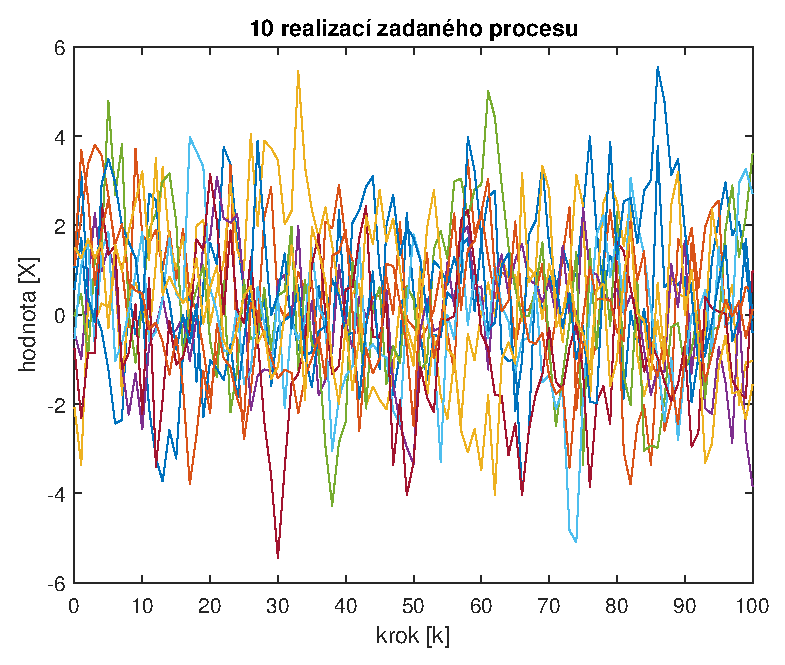
\includegraphics[width=.5\textwidth]{./Graphics/priklad_01_realizace}
				\caption{Prvních \(10\) z celkových \(M=10^{4}\) realizací zadaného Markovského procesu.}
				\label{pic:priklad_01_realizace procesu}
			\end{figure}
			Z rovnice \ref{eqn:odhad_COV_rce} vypočteme odhad kovarianční funkce pro jednotlivé hodnoty \(\tau\) a veškeré realizace \(M\). Získané výsledky srovnáme s teoreticky vypočtenými hodnotami a z grafu \ref{pic:priklad_01_porovnani_kovarianci} je vidět, že se odhadnuté kovariance liší jen málo od teoretických výsledků. Odchylky jsou dány vygenerovaným počtem realizací a pro jejich další zmenšení by bylo nutné zvýšit počet realizací \(M\).
			
			\begin{figure}[H]
				\centering
				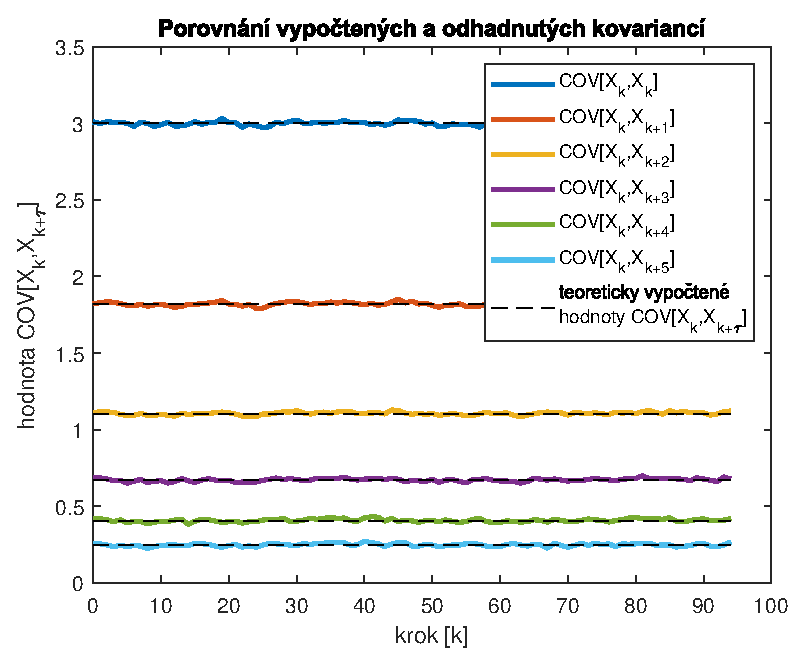
\includegraphics[width=.5\textwidth]{./Graphics/priklad_01_porovnani_kovarianci}
				\caption{Srovnání vypočtených kovariancí s odhadnutými na základě \(M=10^{4}\) realizací procesu.}
				\label{pic:priklad_01_porovnani_kovarianci}
			\end{figure}
		\subsection{Ověření stacionarity procesu}
			Aby byl proces stacionární v širším smyslu, musí splňovat následující kritéria:\\
			
			\noindent
			Střední hodnota procesu \(E[X(t)]\) musí být konstantní pro \(\forall t\).\\
			Ze zadání známe \(E[X_{0}]=0\) a po dopočtení následujících hodnot
			\[E[X_{1}]=e^{-bT}\cdot E[X_{0}]=0\]
			\[E[X_{2}]=e^{-bT}\cdot E[X_{1}]=0\]
			zjistíme, že střední hodnota pro zadaný proces je konstantní s následující hodnotou.
			\[E[X_{k}]=0 ;\forall k\]
			
			Kovarianční funkce musí záviset pouze na rozdílu kroků \(\tau\), což bylo odvozeno a potvrzeno v předešlém úkolu.\\
			
			Zadaný proces tedy splňuje podmínky stacionarity v širším smyslu.
		
	\newpage	
	\section{Příklad č. 2}
		Nyní budeme pracovat s Wienerovým procesem, vygenerujeme jeho 8 realizací a zobrazíme do grafu \ref{pic:priklad_02_realizace_procesu}  
		\begin{figure}[H]
			\centering
			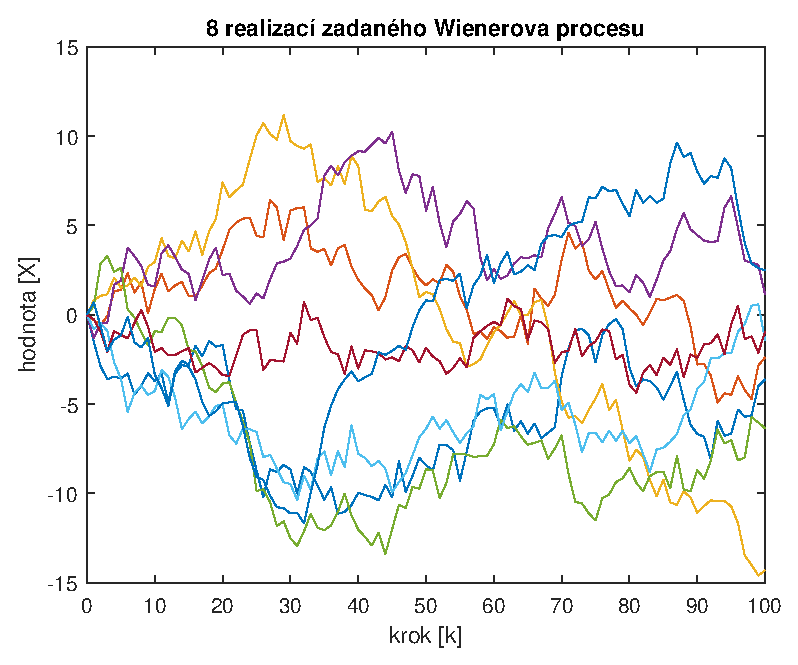
\includegraphics[width=.5\textwidth]{./Graphics/priklad_02_realizace_procesu}
			\caption{8 vykreslených realizací zadaného Wienerova procesu.}
			\label{pic:priklad_02_realizace_procesu}
		\end{figure}
		\subsection{Teoretický výpočet kovariance}
			Jelikož ze zadání neznáme variance a střední hodnoty procesu, které jsou pro výpočet kovariance potřeba, nejprve je vypočteme.
			\begin{align}
				VAR[X_{0}] =& E[X_{0}^{2}]+E[X_{0}]^{2} = E[0^{2}]+ E[0]^{2}=0\\
				VAR[X_{1}] =& VAR[X_{0}+W_{0}] = VAR[X_{0}]+ VAR[W_{0}] = 0 + 1 = 1\\
				VAR[X_{2}] =& VAR[X_{1}+W_{1}] = VAR[X_{1}]+ VAR[W_{1}] = 1 + 1 = 2\\
				\\
				VAR[X_{k}] =& k
			\end{align}
			\begin{align}
				E[X_{0}] =& 0\\
				E[X_{1}] =& E[X_{0}+W_{0}] = E[X_{0}] + E[W_{0}] = 0+0=0\\
				E[X_{2}] =& E[X_{1}] + E[W_{1}] = 0+0=0\\
				\\
				E[X_{k}] = 0
			\end{align}
			Nyní dopočteme kovariance pro pár prvních hodnot \(\tau\) a určíme kovarianční funkci.
			\begin{align}
				COV[X_{k},X_{k}] =& VAR[X_{k}] = k\\
				COV[X_{k},X_{k+1}] =& E[X_{k}\cdot X_{k+1}] + E[X_{k}]\cdot E[X_{k+1}] = E[X_{k}^{2}+X_{k}\cdot W_{k}]+0 = E[X_{k}^{2}]+0=k\\
				\\
				COV[X_{k},X_{k+\tau}] =& E[X_{k}^{2}] = k
			\end{align}
			Z kovarianční funkce lze poznat, že záleží pouze na kroku a nejedná se tedy o stacionární proces, což potvrzuje chování na obrázku \ref{pic:priklad_02_realizace_procesu} a informace v zadání.
		\subsection{Odhad kovarianční funkce}
			Použitím vztahu \ref{eqn:odhad_COV_rce} získáme kovarianční funkci. Vykreslením odhadnuté funkce spolu s teoreticky vypočtenou získáme graf \ref{pic:priklad_02_porovnani_kovarianci}
			\begin{figure}[H]
				\centering
				\includegraphics[width=.5\textwidth]{./Graphics/priklad_02_porovnani_kovarianci}
				\caption{8 vykreslených realizací zadaného Wienerova procesu.}
				\label{pic:priklad_02_porovnani_kovarianci}
			\end{figure}
	\newpage	
	\section{Příklad č. 3}
		Následující výpočty budou uvažovat se zadaným Gauss-Markovým systémem.
		\begin{figure}[H]
			\begin{subfigure}[h]{.5\textwidth}
				\centering
				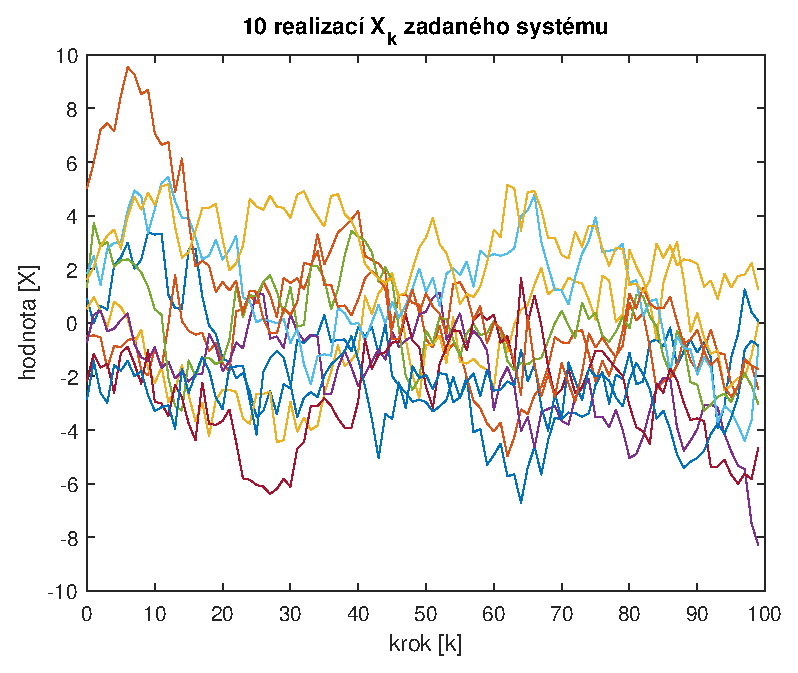
\includegraphics[width=\textwidth]{./Graphics/priklad_03_realizace_procesu_X}
				\caption{Proces \(X_{k}\).}
			\end{subfigure}
			\hfill
			\begin{subfigure}[h]{.5\textwidth}
				\centering
				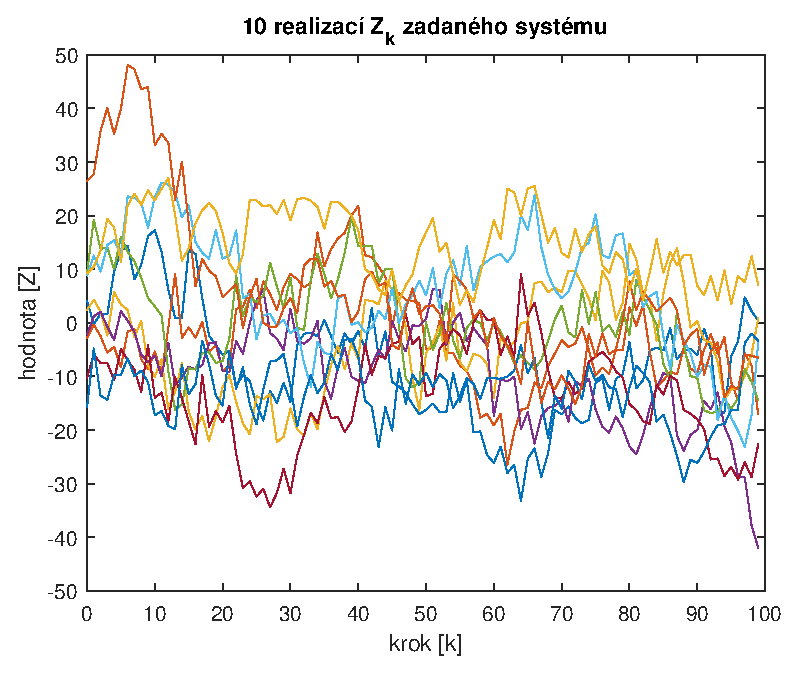
\includegraphics[width=\textwidth]{./Graphics/priklad_03_realizace_procesu_Z}
				\caption{Proces \(Z_{k}\).}
			\end{subfigure}
			\caption{Prvních \(10\) z celkových \(M=10^{4}\) realizací zadaného Gauss-Markova systému.}
			\label{pic:priklad_03_realizace_procesu_X_a_Z}
		\end{figure}
		\subsection{Střední hodnoty}
			Střední hodnoty pro \(X_{k}\)
			\begin{align}
				E[X_{0}] =& 1\\
				E[X_{1}] =& E[0.95\cdot X_{0} + 0.5\cdot W_{0}] = 0.95\cdot E[X_{0}] + 0.5\cdot E[W_{0}] = 0.95 + 0 = 0.95\\
				E[X_{2}] =& E[0.95\cdot X_{1} + 0.5\cdot W_{1}] = 0.95\cdot E[X_{1}] + 0.5\cdot E[W_{1}] = 0.95\cdot 0.95 + 0 = 0.95^{2}\\
				E[X_{3}] =& E[0.95\cdot X_{2} + 0.5\cdot W_{2}] = 0.95\cdot E[X_{2}] + 0.5\cdot E[W_{2}] = 0.95\cdot 0.95^{2} + 0 = 0.95^{3}\\
				\\
				E[X_{k}] =& 0.95^{k}
			\end{align}
		Ustálená hodnota \(\lim\limits_{k\to\infty} E[X_{k}] = \lim\limits_{k\to\infty}0.95^{k}=0\)\\
		Střední hodnoty pro \(Z_{k}\)
			\begin{align}
				E[Z_{0}] =& E[5\cdot X_{0}+V_{0}] = 5\cdot E[X_{0}]+E[V_{0}]= 5\cdot 1 + 0 = 5\\
				E[Z_{1}] =& E[5\cdot X_{1}+V_{1}] = 5\cdot E[X_{1}]+E[V_{1}]= 5\cdot 0.95 + 0 = 5\cdot 0.95\\
				E[Z_{2}] =& E[5\cdot X_{2}+V_{2}] = 5\cdot E[X_{2}]+E[V_{2}]= 5\cdot 0.95^2 + 0 = 5\cdot 0.95^2\\
				\\
				E[Z_{k}] =& 5\cdot 0.95^{k}
			\end{align}
		Ustálená hodnota \(\lim\limits_{k\to\infty} E[Z_{k}] = \lim\limits_{k\to\infty}5\cdot 0.95^{k}=0\)\\
		\subsection{Variance}
			Variance pro \(X_{k}\)
			\begin{align}
				VAR[X_{0}] =& 5\\
				VAR[X_{1}] =& VAR[0.95\cdot X_{0} + 0.5\cdot W_{0}] = 0.95^{2}\cdot VAR[X_{0}] + 0.5^{2}\cdot VAR[W_{0}] = 0.95^{2}\cdot 5 + 0.5^{2}\cdot 3 = 6.25\\
				VAR[X_{2}] =& VAR[0.95\cdot X_{1} + 0.5\cdot W_{1}] = 0.95^2\cdot VAR[X_{1}] + 0.5^2\cdot VAR[W_{1}] = 0.95^{4}\cdot 5 + 0.5^2\cdot 3\cdot (0.95^{2}+1)\\
				VAR[X_{3}] =& VAR[0.95\cdot X_{2} + 0.5\cdot W_{2}] = 0.95^2\cdot VAR[X_{2}] + 0.5^2\cdot VAR[W_{2}] = 0.95^{6}\cdot 5 + 0.5^2\cdot 3\cdot (0.95^{4}+0.95^{2}+1)\\
				\\
				VAR[X_{k}] =& 0.95^{2k}\cdot 5 + 0.5^2\cdot 3\cdot \sum_{n=0}^{k-1}0.95^{2n}
			\end{align}
			Ustálená hodnota \(\lim\limits_{k\to\infty} VAR[X_{k}] = \lim\limits_{k\to\infty}\left(0.95^{2k}\cdot 5\right) + 0.5^2\cdot 3\cdot \lim\limits_{k\to\infty}\left(\sum_{n=0}^{k-1}0.95^{2n}\right)=0+ 0.5^2\cdot 3\cdot \lim\limits_{k\to\infty}\left(\sum_{n=0}^{k-1}0.95^{2n}\right)\)\\
			Pro výpočet druhé limity si však musíme uvědomit, že se jedná o limitu součtu geometrické řady. Zjistíme tedy kvocient \[q=\frac{a_{1}}{a_{0}}=\frac{0.95^{2\cdot1}}{0.95^{2\cdot0}}=0.95^{2}\] a jelikož kvocient \(q=0.95^{2}<1\) geometrická řada konverguje a ustálenou hodnotu dopočteme jako 
			\[\lim\limits_{k\to\infty} VAR[X_{k}]=0+ 0.5^2\cdot 3\cdot \lim\limits_{k\to\infty}\left(\sum_{n=0}^{k-1}0.95^{2n}\right) = 0+ 0.5^2\cdot 3\cdot \frac{a_{0}}{1-q}=0.5^2\cdot 3\cdot \frac{1}{1-0.95^{2}} \approx  7.6923\]\\
			Variance pro \(Z_{k}\)
			\begin{align}
				VAR[Z_{0}] =& VAR[5\cdot X_{0}+V_{0}]= 5^{2}\cdot VAR[X_{0}]+ VAR[V_{0}]=5^{2}\cdot 5 + 2 = 127\\
				\\
				VAR[Z_{k}] =& 5^{2}\cdot VAR[X_{k}] + VAR[V_{k}]
			\end{align}
			Ustálená hodnota \(\lim\limits_{k\to\infty} VAR[Z_{k}] = 5^{2}\cdot \lim\limits_{k\to\infty}VAR[X_{k}] + \lim\limits_{k\to\infty}VAR[V_{k}] = \approx 5^{2}\cdot 7.6923 + 2 \approx 194.3075\)
		\subsection{Porovnání s odhadnutými parametry}
			Na následujících grafech můžeme pozorovat mírné odchylky odhadnutých parametrů od teoreticky vypočtených.
			\begin{figure}[H]
				\begin{subfigure}[h]{.5\textwidth}
					\centering
					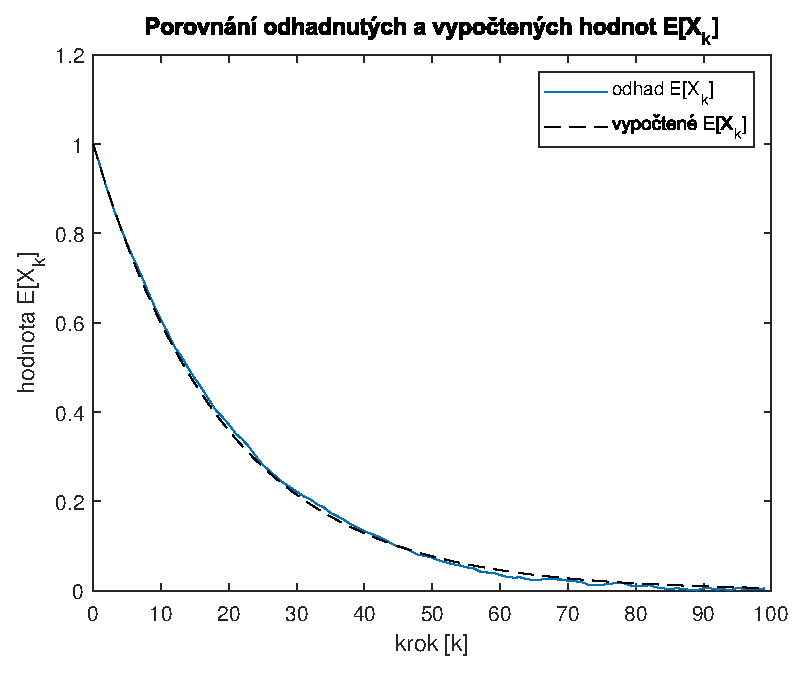
\includegraphics[width=\textwidth]{./Graphics/priklad_03_porovnani_E_X}
					\caption{Průběh \(E[X_{k}]\).}
				\end{subfigure}
				\hfill
				\begin{subfigure}[h]{.5\textwidth}
					\centering
					\includegraphics[width=\textwidth]{./Graphics/priklad_03_porovnani_E_Z}
					\caption{Průběh \(E[Z_{k}]\).}
				\end{subfigure}
				\caption{Porovnání průběhů středních hodnot.}
				\label{pic:priklad_03_porovnani_strednich hodnot}
			\end{figure}
			\begin{figure}[H]
				\begin{subfigure}[h]{.5\textwidth}
					\centering
					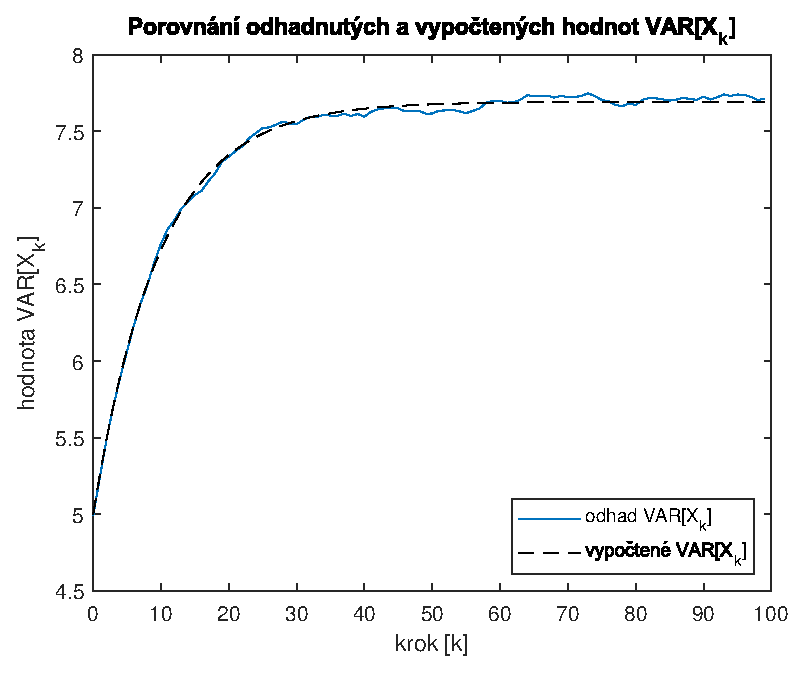
\includegraphics[width=\textwidth]{./Graphics/priklad_03_porovnani_VAR_X}
					\caption{Průběh \(VAR[X_{k}]\).}
				\end{subfigure}
				\hfill
				\begin{subfigure}[h]{.5\textwidth}
					\centering
					\includegraphics[width=\textwidth]{./Graphics/priklad_03_porovnani_VAR_Z}
					\caption{Průběh \(VAR[Z_{k}]\).}
				\end{subfigure}
				\caption{Porovnání průběhů variancí.}
				\label{pic:priklad_03_porovnani_varianci}
			\end{figure}
			U vykreslených grafů \ref{pic:priklad_03_porovnani_strednich hodnot} a \ref{pic:priklad_03_porovnani_varianci} si lze všimnout, že se odhadnuté parametry lehce odlišují od teoreticky vypočítaných hodnot. To je však způsobeno počtem realizací a pro eliminaci nepřesností by muselo být \(M\) realizací velmi mnoho (limitně až \(\infty\)).
	\newpage
	\section{Závěr}
		Vzorce byly čerpány z přednášek a výpočty byly provedeny za pomoci softwaru Matlab. Samotné vypracování práce mi pomohlo lépe pochopit Stochastické procesy, jejich fungování a díky vizualizaci lépe pochopit pojem stacionarita.
\end{document}
